\documentclass[a4paper, 14pt]{extarticle}
\usepackage{./generalPreamble}
\usepackage{./longReportFormat}
\usepackage{./sourceCode}

\newcommand{\Addon}[3]{%
\section*{#1}
\addonsubheader{#2}
\phantomsection{}
\addcontentsline{toc}{section}{#1. #2}
\lstinputlisting[language=C++, style=num]{#3}
}

\usepackage{booktabs}

\usepackage{tocloft}

\begin{document}
    
\begin{titlepage}
    \centering
    {\bfseries
        \uppercase{%
            Минобрнауки России \\
            Санкт-Петербургский государственный \\
            Электротехнический университет \\
            \enquote{ЛЭТИ} им. В.И.Ульянова (Ленина)\\
        }
        Кафедра МО ЭВМ

        \vspace{\fill}
        \uppercase{Лабораторная работа №1} \\
        по дисциплине \enquote{Конструирование ПО} \\
        Тема: Программирование контейнерных классов
    }

    \vspace{\fill}
    \begin{tabularx}{0.8\textwidth}{l X c r}
        Студент гр. 6304 & & \underline{\hspace{3cm}} & Корытов П.В.\\
        Преподаватель & & \underline{\hspace{3cm}} & Спицын А.В.
    \end{tabularx}

    \vspace{1cm}
    Санкт-Петербург \\
    \the\year{}
\end{titlepage}
\newpage
\tableofcontents{}

\newpage

\section{Постановка задачи}
\subsection{Цель работы}
Изучение создания полиморфной иерархии в классов. Разработка контейнера с внешним итератором; изучение контейнеров STL.\@ Изучение отладки и профилирования программ на C++

\subsection{Формулировка задания}
\begin{enumerate}
    \item Разработка программ
    \begin{enumerate}
        \item Настройка среды. Выполнение индивидуального задания
        \begin{itemize}
            \item Индивидуальное задание: Написать классы для создания графических объектов. Классы должны иметь общий абстрактный базовый класс Shape с чистыми виртуальными функциями.
            \item Необходимо использовать множественное наследование. В классах должны быть предусмотрены виртуальные функции для вывода информации об объектах в поток, а Shape должен иметь дружественный перегруженный оператор <<.
            \item Исходный текст должен быть разделен на три файла *.h, *.cpp и *.cpp с тестовой программой.
        \end{itemize}
        \item Работа в режиме отладки.
        \begin{itemize}
            \item Запустить программу и просмотреть ее работу по шагам (Build -> Start Debug -> Go)
            \item Просмотреть иерархию классов и найти примеры множественного наследования.
            \item Расставить точки превывания программы (Break Points) и протестировать её работу.
            \item Для выяснения текущих значений переменных, использовать механизм ``Watch variable''.
        \end{itemize}
        \item Исследование программы при помощи Profiler
        \begin{itemize}
            \item Изучить возможности оптимизации программы в интегрированной среде, в отчете перечислить и объяснить параметры (опции), влияющие на оптимизацию.
            \item Построить несколько вариантов, отличающихся способом оптимизации, проанализировать время работы и объем памяти полученных вариантов. С помощью Profiler определить наиболее долго выполнявшиеся функции. С помощью Profiler определить не исполнявшиеся участки программы.
            \item Изменить текст main так, чтобы выполнялись все участки программы.
        \end{itemize}
    \end{enumerate}
    \item Применение стандартной библиотеки STL
    \begin{enumerate}
        \item Составить консольные приложения, демонстрирующие основные операции с контейнерами и итераторами STL.\@
        \begin{itemize}
            \item Заполняя 3 контейнера строками из <cstring> или другими элементами, продемонстрировать отличия
            \begin{itemize}
                \item последовательностей (vector, list, dequeue);
                \item адаптеров последовательностей (stack, queue, priority\_queue);
                \item ассоциативных контейнеров на базе map.
            \end{itemize}
            \item На примере заполнения одного контейнера-последовательности из предыдущего задания целыми числами, протестировать интерфейсы контейнера и итератора.
            \item Аналогично протестировать ассоциативный контейнер, заполняя его указателями на разные графические объекты. Протестировать алгоритмы-методы и алгоритмы-классы на множестве графических элементов.
        \end{itemize}
        \item Реализовать новый шаблон контейнера и шаблон итератора для него по индивидуальному заданию.
        \begin{itemize}
            \item Предусмотреть обработку исключительных ситуаций.
            \item Протестировать контейнер, заполнив его графическими объектами.
            \item В отчете формально описать реализуемую структуру данных и абстракцию итерации, перечислить все отношения между классами, описать интерфейсы классов и особенности реализации.
        \end{itemize}
    \end{enumerate}
\end{enumerate}

\section{Ход работы}
Использованное ПО
\begin{enumerate}
    \item \textbf{JetBrains CLion} --- IDE для C/C++
    \item \textbf{Valgrind} --- проверка утечек памяти
    \item \textbf{Google Test} --- юнит-тесты для C++ 
    \item \XeLaTeX{}, \textbf{neovim} --- сборка и написание отчёта 
\end{enumerate}

\subsection{Создание классов фигур}
\begin{enumerate}
    \item Создан класс Point (файлы point.h, point.cpp). Он содержит основные математические операции по работе с точками, например конвертацию координат.
    \item Создан общий абстрактный класс Shape (shape.h, shape.cpp). Он содержит базовые методы, необходимые всем фигурам, несколько виртуальных и чистых виртуальных методов.\\
    Оператор вывода в поток не виртуальный, т.к. дружественные методы не наследуются. Вместо этого в операторе вызывается чистый виртуальный метод print, который является protected и может наследоваться.
    \item Написаны классы Pentagram, AtanSegment, Text, PentagramText. Класс PentagramText наследуется от Pentagram и Text. UML-диаграмма классов представлена на рисунке~\ref{img:uml:shapes}.

    Исходные коды представлены в приложениях в соответствующих файлах
    \begin{figure}[h]
        \centering
        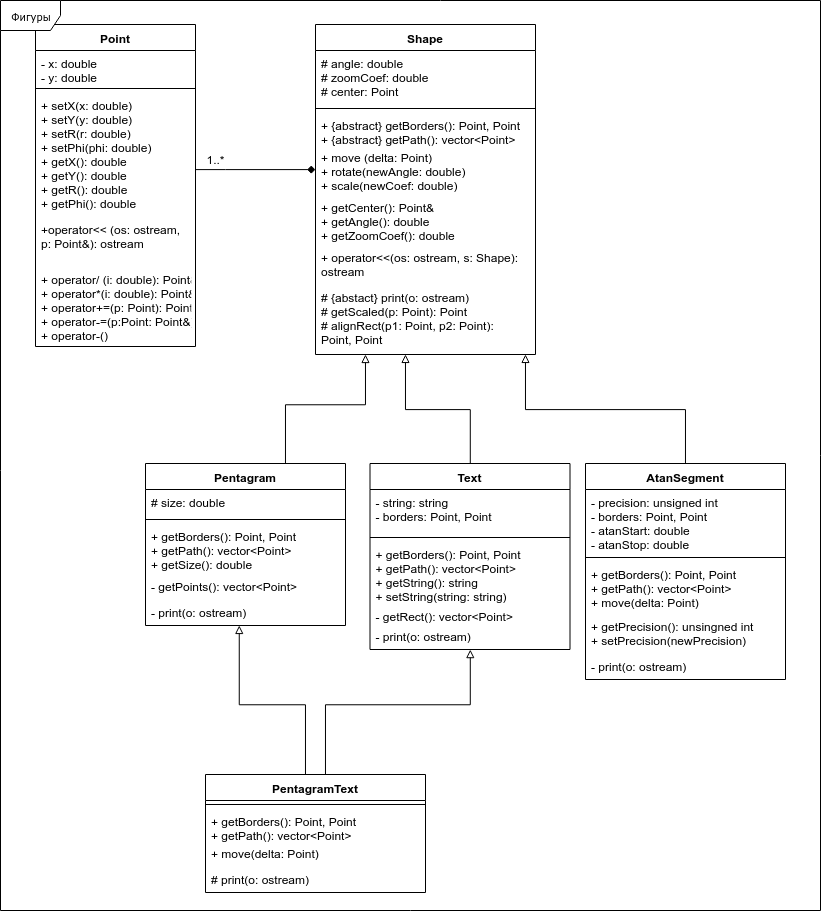
\includegraphics[width=\textwidth]{./img/classes_uml.png}
        \caption{UML-диаграмма классов}%
        \label{img:uml:shapes}
    \end{figure}
\end{enumerate}

\FloatBarrier{}
\subsection{Проверка созданных классов}
\begin{enumerate}
    \item Для тестирования созданных классов подключен фреймворк GoogleTest, написан ряд юнит-тестов. Исходный код тестов находится в test.cpp.\\
    Процесс запуска юнит-тестов представлен на~\ref{img:shapes:tests}
    \begin{figure}[h]
        \centering
        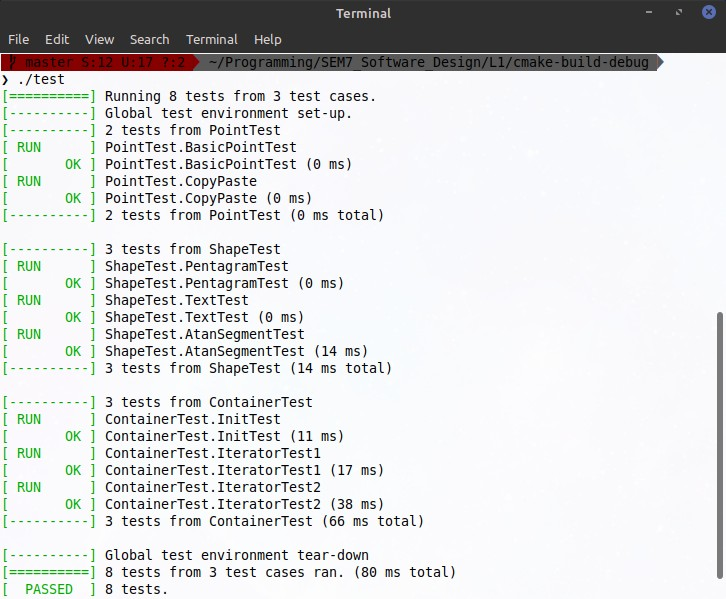
\includegraphics[width=0.8\textwidth]{./img/S001.jpg}
        \caption{Запуск Google Tests}%
        \label{img:shapes:tests}
    \end{figure}
    \item Для демонстрации написан ряд преобразований над фигурами. Код преобразований в файле demo.cpp. Ход преобразований представлен на рисунке~\ref{img:shapes:demo}
    \begin{figure}[h]
        \centering
        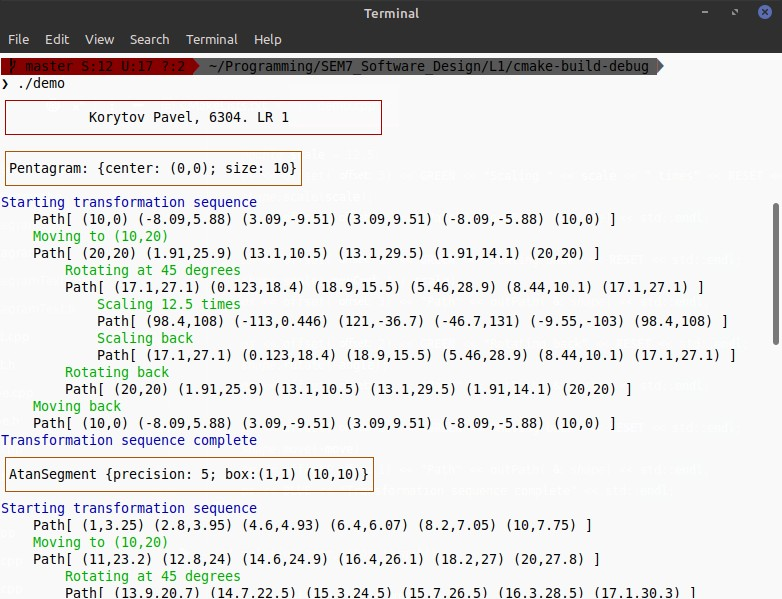
\includegraphics[width=0.8\textwidth]{./img/S002.jpg}
        \caption{Запуск преобразований}%
        \label{img:shapes:demo}
    \end{figure}
    
    Преобразования над всеми фигурами выполнены корректно.

    \item Для отладки использована обертка над gdb, встроенная в CLion и Valgrind для контроля над утечками памяти.
    Приведены скриншоты, сделанные в ходе отладки:
    \begin{itemize}
        \item Рисунок~\ref{img:shapes:breakpoint} --- остановка на breakpoint'e
        \begin{figure}[h]
            \centering
            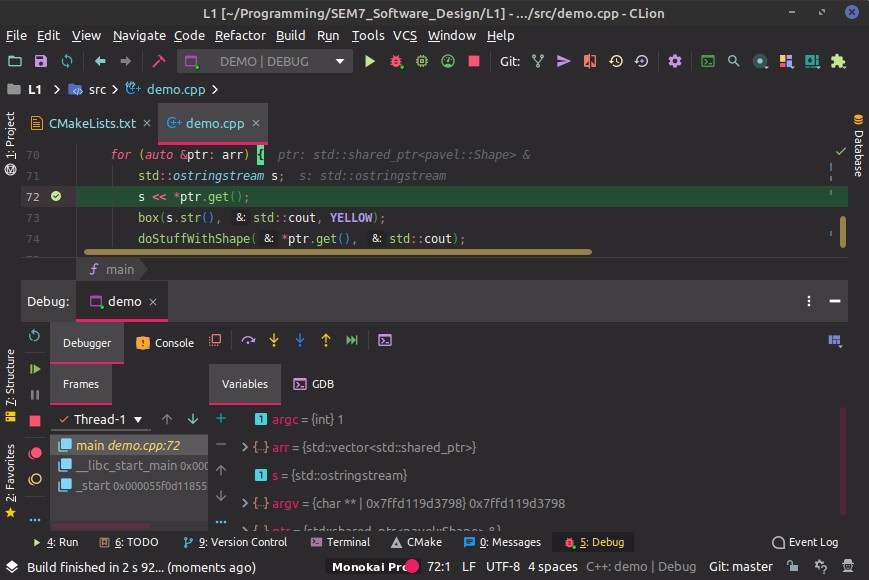
\includegraphics[width=\textwidth]{./img/S003.jpg}
            \caption{Остановка на breakpoint'е}%
            \label{img:shapes:breakpoint}
        \end{figure}
        \item Рисунок~\ref{img:shapes:eval} --- оценка выражения
        \begin{figure}[h]
            \centering
            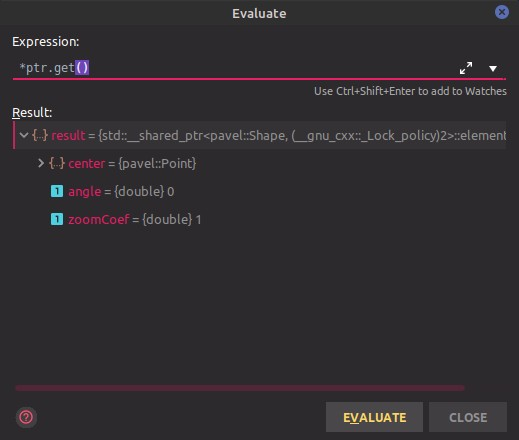
\includegraphics[width=0.7\textwidth]{./img/S004.jpg}
            \caption{Оценка значения выражения}%
            \label{img:shapes:eval}
        \end{figure}
        \item Рисунок~\ref{img:shapes:leak} --- локализация утечки памяти
        \begin{figure}[h]
            \centering
            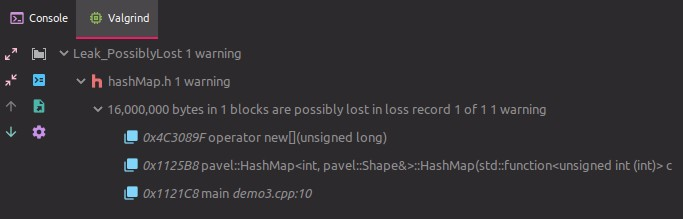
\includegraphics[width=\textwidth]{./img/S005.jpg}
            \caption{Valgrind обнаружил утечку памяти}%
            \label{img:shapes:leak}
        \end{figure}
    \end{itemize}
    \FloatBarrier{}
\end{enumerate}

\FloatBarrier{}
\subsection{Применение стандартной библиотеки STL}
\begin{itemize}
    \item Составлено консольное приложение, демонстрирующее различия между различными контенерами STL.\@ Код в demo2.cpp.
    
    Установлено, что хотя интерфейсы контейнеров очень похожи, эффективность различных операций в них различается.

    \begin{figure}[h]
        \centering
        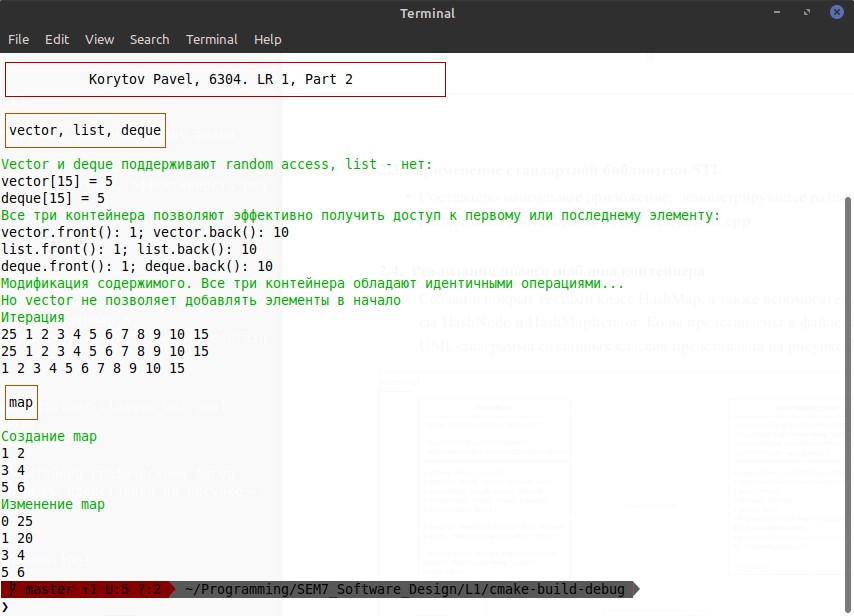
\includegraphics[width=\textwidth]{./img/S010.jpg}
        \caption{Результаты запуска демострационной программы}%
        \label{img:stl:demo}
    \end{figure}

    Некоторые различия между vector, list и deque указаны в таблице~\ref{tab:stl:diff}.
    \begin{table}[h]
        \centering
        \caption{Различия между контейнерами}
        \begin{tabular}{@{}llll@{}}
        \toprule
        \textbf{Метод} & \textit{std::vector} & \textit{std::list} & \textit{std::deque} \\ \midrule
        Доступ по индексу & + & --- & + \\
        Доступ с начала / конца & + & + & + \\ \midrule
        Добавление элементов в конец & + & + & + \\
        Добавление элементов в начало & --- & + & + \\
        Изменение элементов по индексу & + & --- & + \\ \bottomrule
        \end{tabular}%
        \label{tab:stl:diff}
    \end{table}

\end{itemize}

\subsection{Реализация нового шаблона контейнера}
\begin{enumerate}
    \item Создан и покрыт тестами класс HashMap, а также вспомогательные классы HashNode и HashMapIterator. Коды представлены в файле hashMap.h.
    UML-диаграмма созданных классов представлена на рисунке~\ref{img:uml:container}
    \begin{figure}[h]
        \centering
        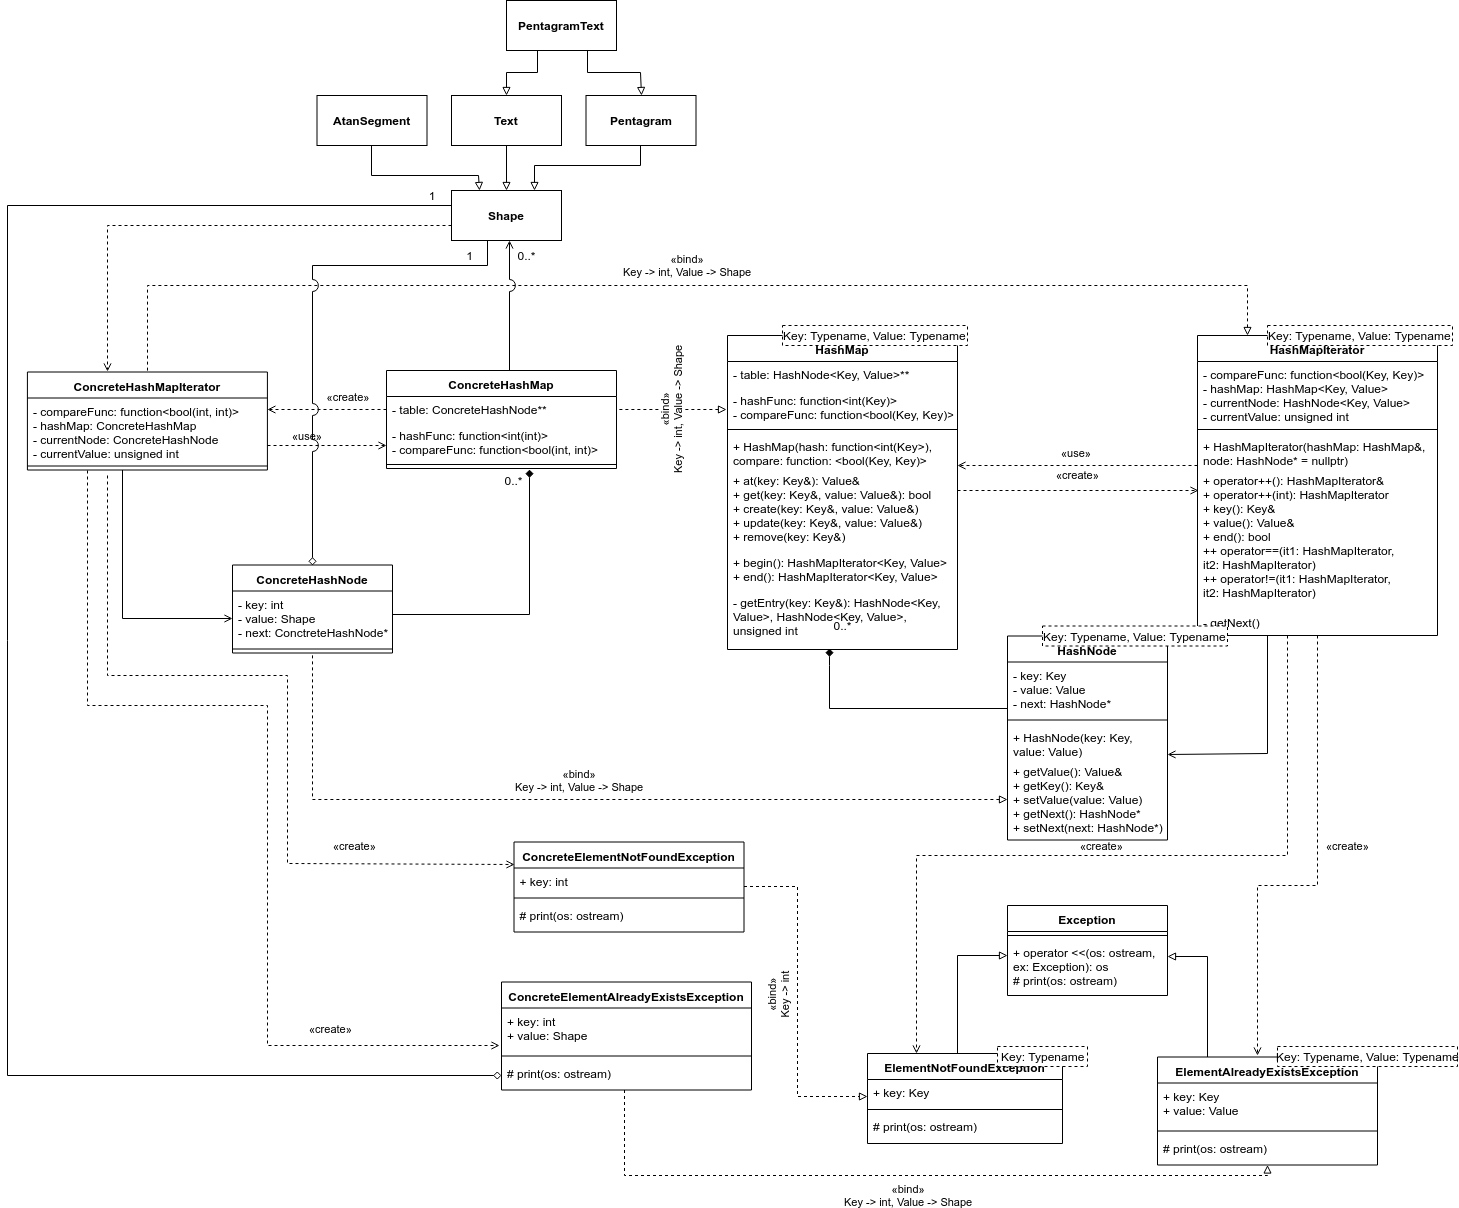
\includegraphics[width=\textwidth]{./img/container_classes_uml.png}
        \caption{UML-диаграмма классов контейнера}%
        \label{img:uml:container}
    \end{figure}
    \item Создано приложение, заполняющее созданный контейнер графическими фигурами. Код в demo3.cpp. Запуск демонстрацинной программы представлен на рисунке~\ref{img:map:demo}
    \begin{figure}[h]
        \centering
        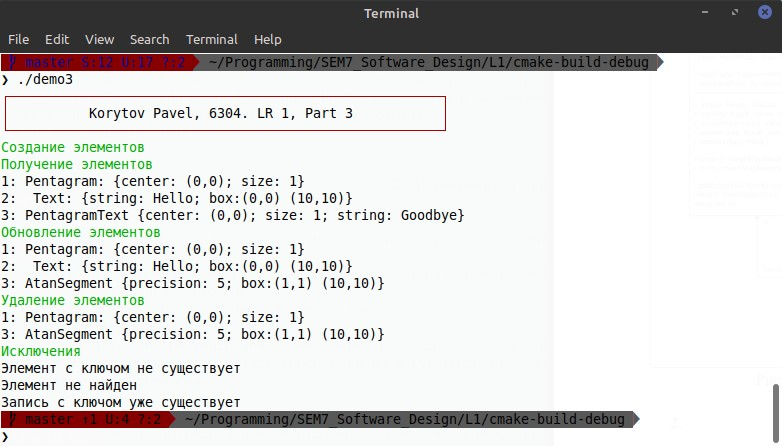
\includegraphics[width=\textwidth]{./img/S006.jpg}
        \caption{Запуск демострации HashMap}%
        \label{img:map:demo}
    \end{figure}

    \item Изучение профилировщика\\
    Использована обёртка над профилировщиком Perf, встроенная в CLion.

    На рисунке~\ref{img:map:calltree} --- дерево вызовов, на~\ref{img:map:methods} --- вызываемые методы

    \begin{figure}[h]
        \centering
        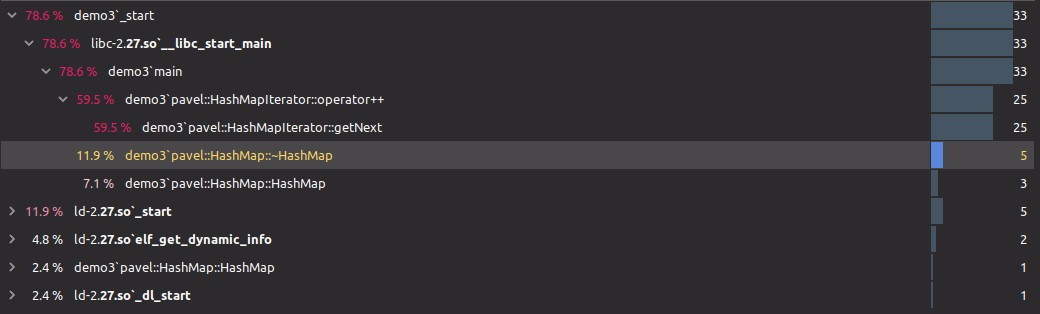
\includegraphics[width=\textwidth]{./img/S008.jpg}
        \caption{Дерево вызовов}%
        \label{img:map:calltree}
    \end{figure}
    
    \begin{figure}[h]
        \centering
        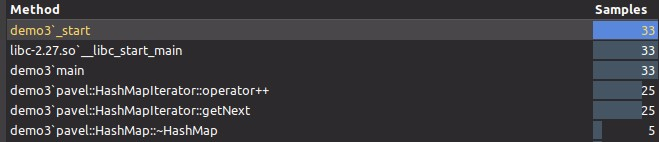
\includegraphics[width=\textwidth]{./img/S009.jpg}
        \caption{Список вызываемых методов}%
        \label{img:map:methods}
    \end{figure}
    
    

    
\end{enumerate}
\section{Выводы}
Протестированы и изучены классы контейнеров стандартной библиотеки STL.\@ 

Написаны классы графических объектов, поддерживающие полиморфизм. Изучено виртуальное наследование для разрешения проблем, связанных с ромбовидным наследованием.

Написан класс-контейнер --- хэш-таблица на базе списка.


\Addon{Приложение А}{Код shape.h}{../src/figures/shape.h}
\Addon{Приложение Б}{Код shape.cpp}{../src/figures/shape.cpp}
\Addon{Приложение В}{Код point.h}{../src/figures/point.h}
\Addon{Приложение Г}{Код point.cpp}{../src/figures/point.cpp}
\Addon{Приложение Д}{Код pentagram.h}{../src/figures/pentagram.h}
\Addon{Приложение Е}{Код pentagram.cpp}{../src/figures/pentagram.cpp}
\Addon{Приложение Ж}{Код atanSegment.h}{../src/figures/atanSegment.h}
\Addon{Приложение З}{Код atanSegment.cpp}{../src/figures/atanSegment.cpp}
\Addon{Приложение И}{Код text.h}{../src/figures/text.h}
\Addon{Приложение К}{Код text.cpp}{../src/figures/text.cpp}
\Addon{Приложение Л}{Код pentagramText.h}{../src/figures/pentagramText.h}
\Addon{Приложение М}{Код pentagramText.cpp}{../src/figures/pentagramText.cpp}
\Addon{Приложение Н}{Код test.cpp}{../src/test.cpp}
\Addon{Приложение О}{Код demo.cpp}{../src/demo.cpp}
\Addon{Приложение П}{Код colors.h}{../src/colors.h}
\Addon{Приложение Р}{Код myCli.h}{../src/cli/myCli.h}
\Addon{Приложение С}{Код myCli.cpp}{../src/cli/myCli.cpp}
\Addon{Приложение Т}{Код demo2.cpp}{../src/demo2.cpp}
\Addon{Приложение У}{Код hashMap.h}{../src/container/hashMap.h}
\Addon{Приложение Ф}{Код demo3.cpp}{../src/demo3.cpp}


\end{document}
